\documentclass[12pt]{extarticle}
\usepackage[margin=3cm, footskip=55pt]{geometry}
\usepackage{fancyhdr}
\usepackage{titling}
\usepackage{filecontents}
\usepackage{multicol}
\usepackage{graphicx}

\setlength{\droptitle}{-7em} 
\pagestyle{empty}
\pagestyle{fancy}
\fancyhf{}
\renewcommand{\headrulewidth}{0pt}
\lfoot{CMPT 330 Assign 2}
\rfoot{Page: \thepage}
\title{CMPT 330 Assign 2}
\author{Tyler Kuipers}
\date{\today}
\graphicspath{ {./} }
\fancypagestyle{plain}{%
	\renewcommand{\headrulewidth}{0pt}%
	\fancyhf{}%
	\lfoot{CMPT330 Assign 2}
	\rfoot{Page: \thepage}
	% \fancyfoot[C]{\footnotesize Page \thepage\ of \pageref{LastPage}}%
}

\begin{document}
	\maketitle

	\section*{Question 1}
		In the example given, they are named the same thing because in C, there is a library that wraps all of the system calls, and for the sake of simplicity, they are called the same thing.  It is not essential that both of these things have the same name, but it is helpful that they do.  The system call is the more important of the two because it can put the system into kernel mode, while the library call cannot.

	\section*{Question 2}
		Interrupt handlers are written at least in part in assembly because when the interrupt happens, the operating system will give control to the process that was interrupted for.  After this process completes, the stack and registers must be restored back to the state they were in before the interrupt.  Manipulating the stack and registers is extremely difficult in C, and so you need to use a lower level language.

	\section*{Question 3}  
		Modern operating systems segregate the kernel stack and the user stack to prevent bugs.  If someone is not careful with their memory management and starts to overwrite other parts of the stack, it could cause a lot more damage if they are overwriting the kernel part of the stack as opposed to the user part of the stack.

	\section*{Question 4}
		Line 42 - Is a system call.  Printf uses the call write to push it's information into stdout.\\
		Line 43 - Non-Instruction.  Whitespace\\
		Line 44 - Built-in Operation.  This comparison operation is built into the C language, and just compares the next thing in the linked list to null.\\
		Line 45 - Is a system call.  Printf uses the call write to push it's information into stdout.\\
		Line 46 - Is a system call.  fwrite uses the call write to push it's information into the file writing buffer.\\
		Line 47 - Is a system call.  Printf uses the call write to push it's information into stdout.\\
		Line 48 - Is a system call.  Stops the execution of the current process.\\
		Line 49 - Non-Instruction.  Just there for the sake of syntax\\
		Line 50 - Non-Instruction.  Whitespace\\
		Line 51 - Built-in Operation.  This just changes where the byteCache pointer is pointing.\\
		Line 52 - Built-in Operation.  This just changes where the currentByte pointer is pointing.\\
		Line 53 - Non-Instruction.  Whitespace\\
		Line 54 - Built-in Operation.  free() and malloc() are two standard C library functions.\\
		Line 55 - Non-Instruction.  Just there for the sake of syntax\\
		Line 56 - Non-Instruction.  Whitespace\\
		Line 57 - Built-in Operation.  free() and malloc() are two standard C library functions.\\
		Line 58 - Non-Instruction.  Whitespace\\
		Line 59 - Is a system call.  Printf uses the call write to push it's information into stdout.\\

		It is important that a user understand which procedures produce a system call because we should be able to understand where our program gets trapped and how the c library is implemented within our OS.

	\section*{Question 5}
		\begin{enumerate}
			\item Running -\textgreater Blocked.  The OS takes CPU time from one process and blocks it.
			\item Blocked -\textgreater Running.  The OS gives CPU time to a process.
			\item Ready -\textgreater Blocked.  A program is ready but the CPU blocks it in favour of another program.
			\item Blocked -\textgreater Ready.  A program is block and the gets an interrupt and is ready.
			\item Running -\textgreater Ready.  Not Possible.
			\item Ready -\textgreater Running.  A program is ready and is then given CPU time.
		\end{enumerate}
	\clearpage
	\section*{Question 6}
		You have 4 processes each taking a total time of 15 ms.  A multiprogramming system allows us to run multiple programs at the `same' time.  
		\begin{enumerate}
			\item Each process waits for I/O 50\% of the time
				\begin{enumerate}
					\item In a sequential system, this will take a total of 60ms CPU time, plus another 30ms I/O time.  90ms
					\item In a multiprogramming system, this will take a total of 60 ms CPU time, while waiting for I/O 30ms.  Because of multiprogramming, we can negate the I/O time because another process will run while the first is waiting. 60ms
				\end{enumerate}
				This gives us a speedup of 90/60 or 1.5
			\item Each process waits for I/O 75\% of the time
				\begin{enumerate}
					\item In a sequential system, this will take a total of 60ms CPU time, plus another 45ms I/O time. 105ms
					\item In a multiprogramming system, this will take a total of 60 ms CPU time, while waiting for I/O 45ms.  Because of multiprogramming, we can negate the I/O time because another process will run while the first is waiting. 60ms
				\end{enumerate}
				This gives us a speedup of 105/60 or 1.75.
			\item Each process waits for I/O 25\% of the time
				\begin{enumerate}
					\item In a sequential system, this will take a total of 60ms CPU time, plus another 15ms I/O time. 75ms
					\item In a multiprogramming system, this will take a total of 60 ms CPU time, while waiting for I/O 15ms.  Because of multiprogramming, we can negate the I/O time because another process will run while the first is waiting. 60ms
				\end{enumerate}
				This gives us a speedup of 75/60 or 1.25\\
				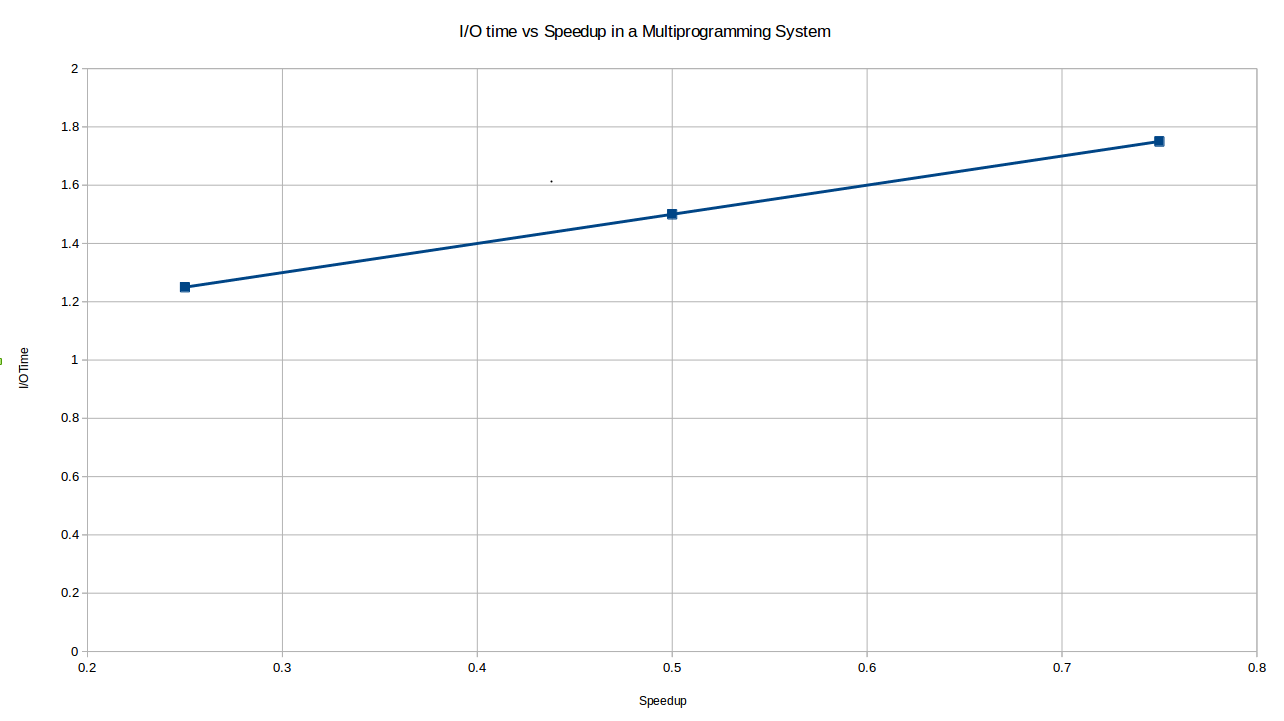
\includegraphics[width=15cm,height=10cm]{pic}\\
				You can see that the speedup gets greater as the I/O time gets higher.  It follows that once the program has a longer I/O wait time than their CPU time, the speedup will be lost because then the CPU will have nothing else to do.
		\end{enumerate}


\end{document} 